\chapter{Validazione sperimentale}
La presente sezione è dedicata alla presentazione dei risultati ottenuti attraverso una serie di test sperimentali. Vengono descritte le diverse prove effettuate e le criticità riscontrate durante il loro svolgimento.

\section{Controllo}
La prima fase sperimentale è stata dedicata alla verifica funzionale dei driver e del nodo ROS forniti da AgileX per il rover modello Hunter. L'obiettivo primario era determinare se tali componenti, specificamente progettati per il controllo e l'analisi del veicolo, potessero essere integrati nel sistema senza richiedere modifiche sostanziali o se, al contrario, fosse necessario apportare adattamenti o addirittura una completa riscrittura.

\noindent Per condurre questa valutazione, è stato sviluppato un nodo ROS dedicato alla ricezione dei dati da un joystick. Questi dati, dopo un'elaborazione preliminare, venivano convertiti in un angolo di sterzo e una velocità che, successivamente, venivano pubblicati sul topic ROS \textit{/drive\_parameters} sotto forma di messaggi di tipo Ackermann. Tale configurazione consentiva di verificare direttamente:

\begin{itemize}
  \item Compatibilità del nodo ROS AgileX: se il nodo ROS fornito dal produttore supportasse il formato dei messaggi Ackermann, comunemente utilizzato per il controllo di veicoli mobili
  \item Efficacia del driver: se il driver fosse in grado di tradurre correttamente i messaggi ROS in messaggi CAN, permettendo così al rover di eseguire i comandi impartiti
\end{itemize}

\noindent I primi test non sono andati a buon fine in quanto, dopo un'accurata analisi, si è riscontrato che il nodo ROS di casa AgileX utilizza un diverso formato di messaggi per il controllo del mezzo, interrompendo così lo stack.

\noindent La soluzione che si è deciso di adottare è stata di introdurre una modifica puntuale al nodo ROS AgileX. Tale modifica ha consentito al nodo di interpretare correttamente il tipo di messaggi previsto, ripristinando così la compatibilità con il resto del sistema

\section{Mappatura}
Il secondo test è stato quello di eseguire una mappatura bidimensionale di un intero ambiente.

\noindent Con mappatura bidimensionale si intende ricreare una vista dall'alto di un ambiente grazie all'utilizzo del sensore Lidar e dell'odometria del mezzo. Conoscendo infatti lo spostamento e la pointcloud rilevata dal sensore, tramite un apposito algoritmo è possibile ricreare questa mappa.

\noindent Per realizzare questa operazione, è stato impiegato un algoritmo di Simultaneous Localization and Mapping (SLAM). Come suggerisce il nome, lo SLAM è una tecnica che consente di localizzare un robot all'interno di un ambiente sconosciuto e, contemporaneamente, di costruire una mappa di tale ambiente. In questo caso specifico, l'algoritmo SLAM è stato implementato nel nodo ROS \textbf{slam\_toolbox}, un pacchetto software open-source ampiamente utilizzato nella comunità robotica.

\noindent Dopo una fase di configurazione iniziale e alcune prove preliminari, è stato possibile generare una mappa bidimensionale accurata del primo piano dell'edificio di matematica del Dipartimento di Scienze Fisiche, Matematiche e Informatiche dell'Università di Modena e Reggio Emilia (UNIMORE). La mappa ottenuta rappresenta una fedele rappresentazione planimetrica dell'ambiente, evidenziando con precisione gli ostacoli presenti e le caratteristiche geometriche delle pareti

\noindent La mappa ottenuta grazie a questi test è riportata in figura \ref{franco_map}.

\begin{figure}[H]
  \centering
  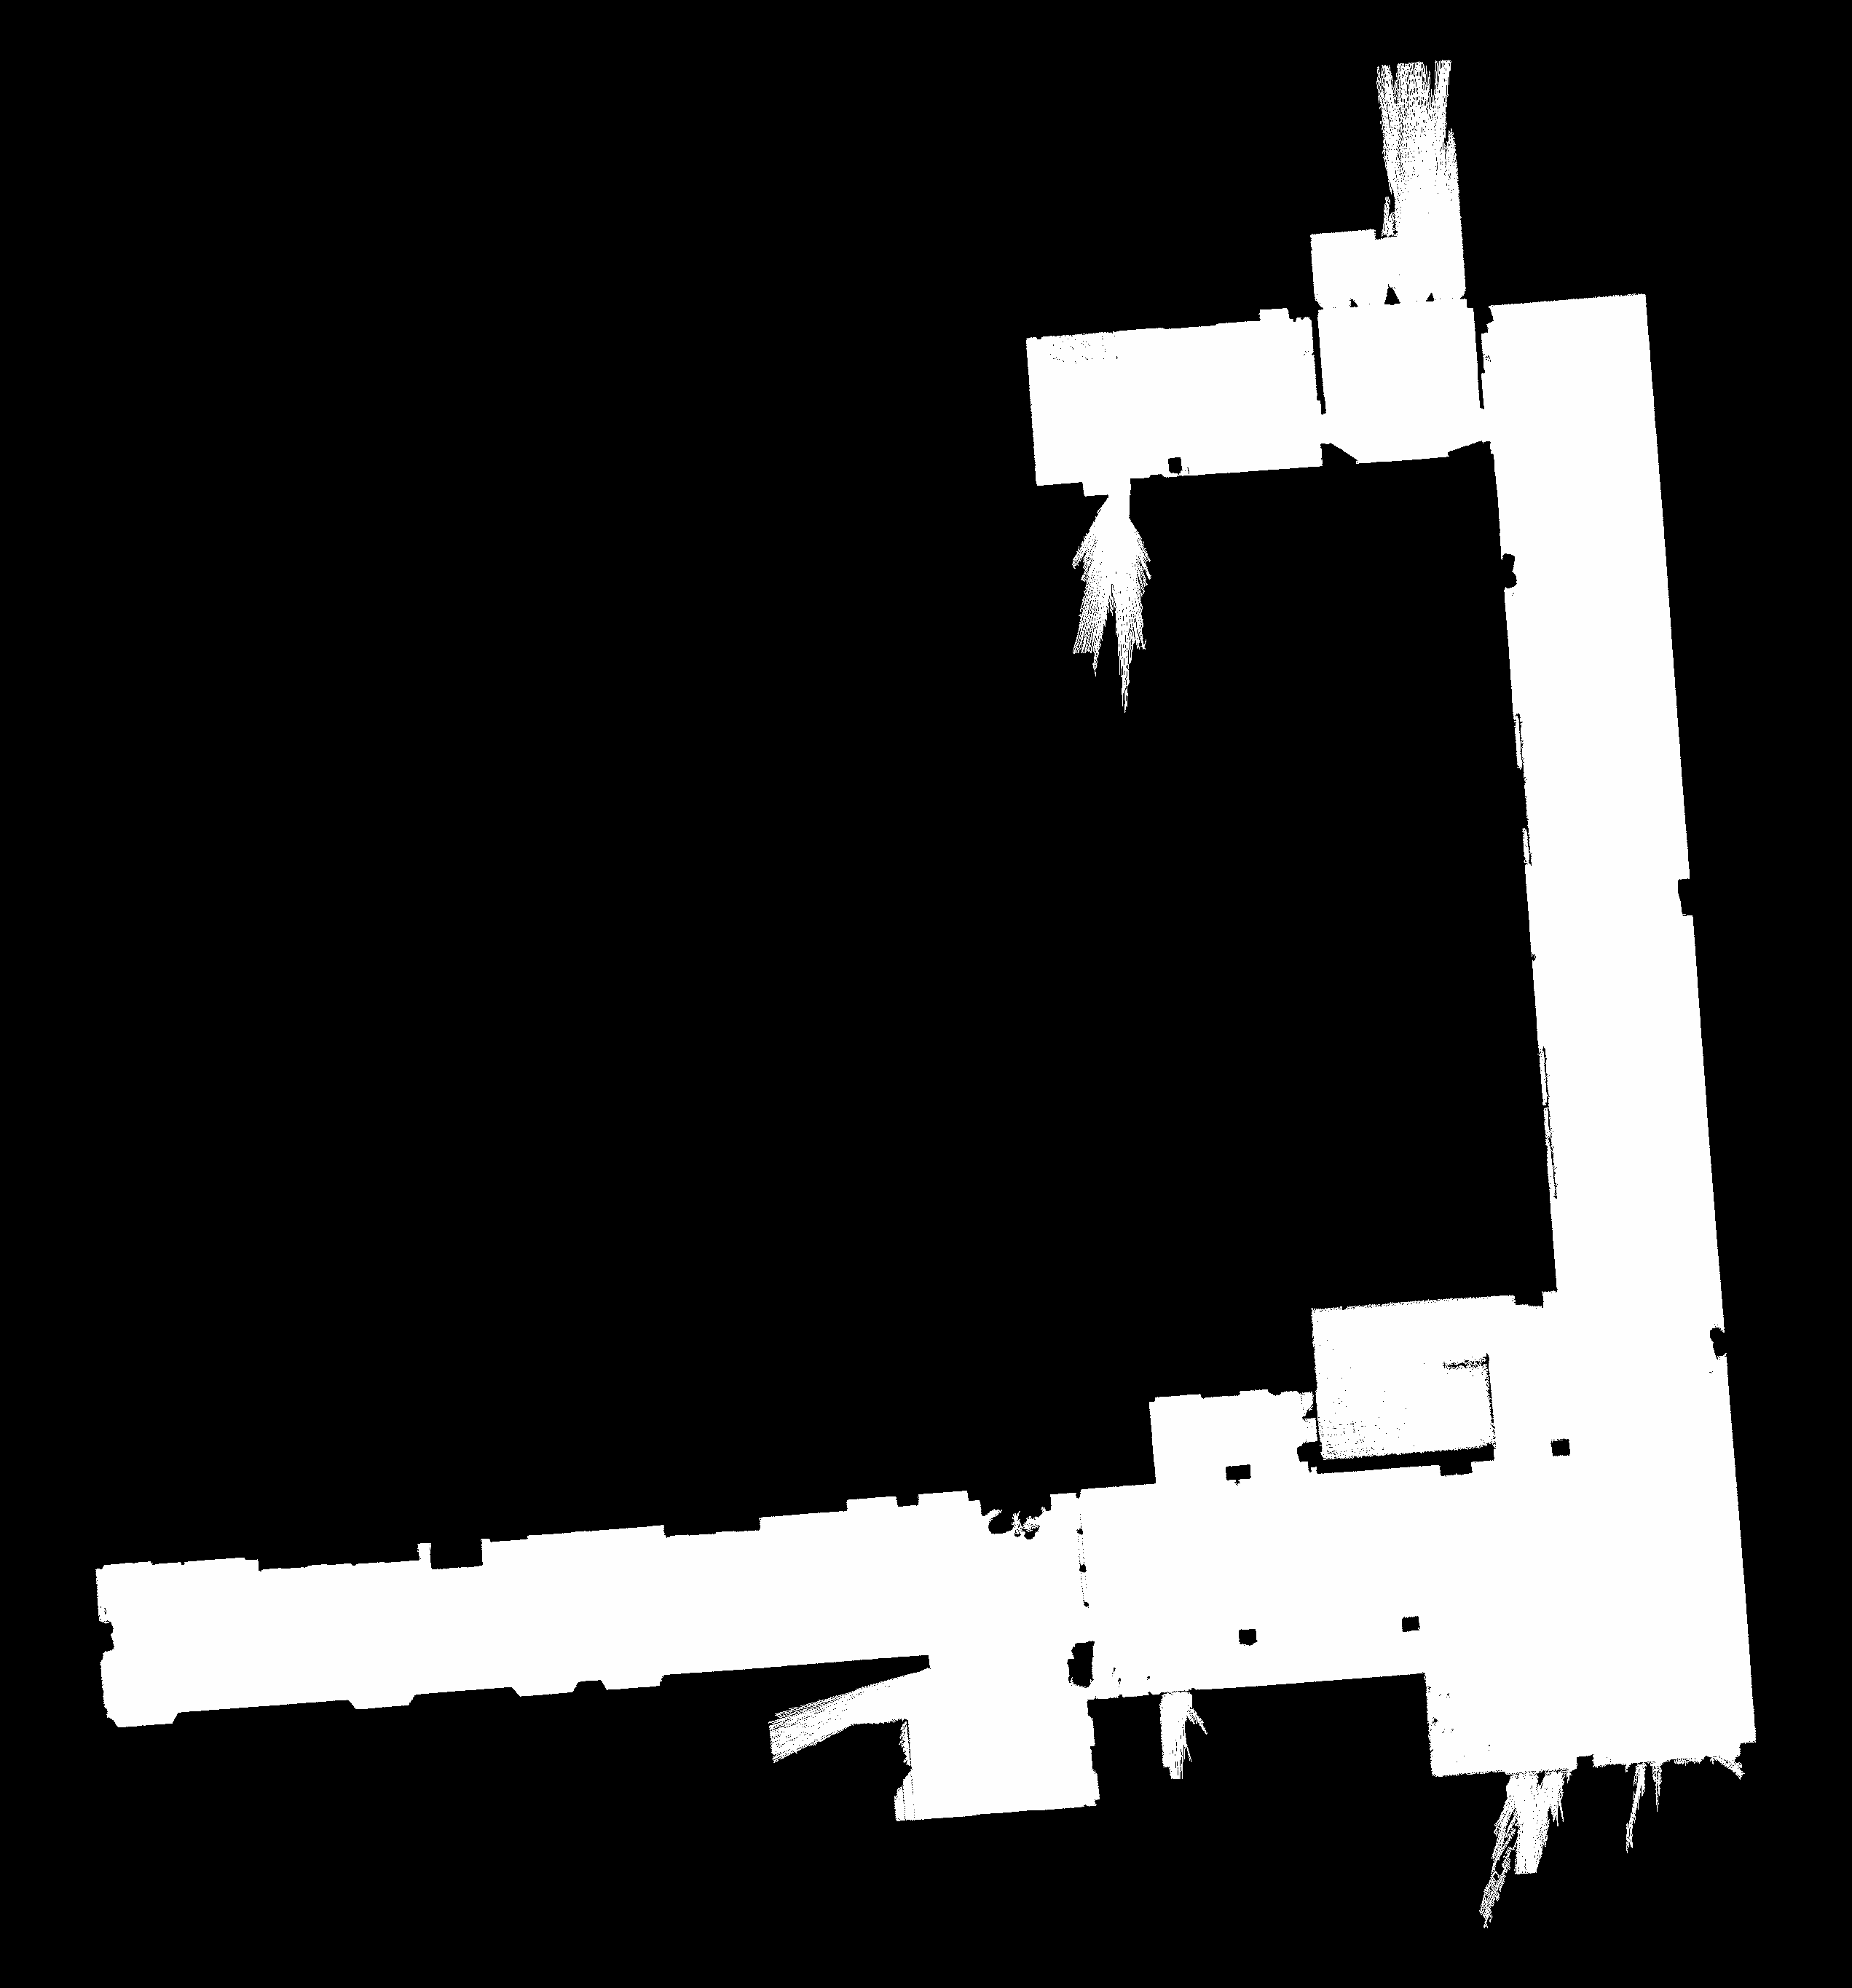
\includegraphics[width=0.5\textwidth]{figures/franco_map.png}
  \caption{Mappa ottenuta tramite Lidar del primo piano dell'edificio Matematica}
  \label{franco_map}
\end{figure}

\section{Localizzazione}
Il terzo test è stato uno dei più importanti, e riguarda la localizzazione.

\noindent Avendo una mappa dell'ambiente grazie ai test precedenti è stato infatti possibile svolgere test volti al calcolo preciso della propria posizione all'interno di un ambiente conosciuto. Questi test sono stati svolti grazie al nodo ROS \textbf{particle\_filter} che implementa l'algoritmo di localizzazione già discusso alla sezione \ref{funzionamento_autonomo_perception}.

\noindent I test di localizzazione condotti hanno evidenziato alcune criticità legate alla natura dell'ambiente di prova. In particolare, sono state riscontrate difficoltà nel raggiungimento di una stima accurata della posizione in determinate aree dell'ambiente, caratterizzate da una scarsità di elementi distintivi (featureless). Tale condizione ha limitato la capacità del filtro a particelle di discriminare tra posizioni potenzialmente simili, compromettendo così la precisione della localizzazione.

\noindent Una soluzione a questo problema può essere sicuramente quella di utilizzare un Lidar più avanzato a tre dimensioni, in modo da apprezzare feature dell'ambiente che non sarebbero altrimenti rilevabili in due dimensioni, soluzione che sta venendo sperimentata al momento della stesura della presente tesi.

\section{Guida autonoma}
La penultima sperimentazione ha avuto come obiettivo la verifica delle prestazioni complessive del sistema di navigazione autonoma. A partire dalla mappa dell'ambiente generata precedentemente e dai parametri di controllo ottimizzati, è stato pianificato un percorso di riferimento. Successivamente, il robot è stato incaricato di seguire il percorso predefinito, utilizzando l'algoritmo di localizzazione per stimare la propria posizione in tempo reale e adattare la traiettoria in base alle informazioni sensoriali acquisite.

\noindent Sebbene i risultati ottenuti siano stati generalmente positivi, si sono manifestati alcuni problemi di deviazione dalla traiettoria pianificata, attribuibili alle incertezze nella stima di posizione e particolarmente evidenti nelle aree dell'ambiente prive di elementi distintivi.

\section{Guida remota}
In conclusione, sono stati svolti test per quanto concerne la guida remota. Nello specifico si è utilizzato un gamepad connesso ad un computer portatile che andasse a comunicare con il nodo ROS \textit{mqtt\_server\_node} per l'impartizione e per l'invio dei comandi tramite rete. Contemporaneamente, sul veicolo venivano eseguiti i nodi \textbf{mqtt\_control\_node} per la ricezione dei comandi e \textbf{hunter\_ros2\_node} per inviare i comandi all'interfaccia CAN del veicolo.

\noindent Per la comunicazione MQTT è stato utilizzato un broker accessibile da rete pubblica con cui sia il veicolo che il portatile (che nell'esperimento rappresentava il server) andavano a comunicare. 

\noindent Le verifiche effettuate hanno confermato il corretto funzionamento degli applicativi, sebbene abbiano messo in luce alcune inefficienze. Tra queste, la latenza nella comunicazione tra veicolo e stazione di controllo è risultata particolarmente critica. Il tempo di risposta, misurato tra l'invio di un comando dal gamepad e la corrispondente azione del veicolo, ha mostrato valori elevati, rendendo l'applicazione non idonea a scenari che richiedono tempi di reazione rapidi come la guida remota.

\section{Latenza}
Successivamente ai test di guida remota sono stati eseguite delle misurazioni di invio e ricezione dei pacchetti per verificare la latenza generata dallo stack. 

\noindent Per facilitare la ripetibilità e l'analisi dei dati, durante i test di guida autonoma sono stati generati diversi file rosbag, ovvero file eseguibili contenenti una registrazione completa dei messaggi scambiati tra i nodi del sistema ROS durante la loro esecuzione. Grazie a questa risorsa, è stato possibile condurre multiple iterazioni di test sulla latenza senza la necessità di rieseguire fisicamente le manovre del rover.

\noindent Le misurazioni di latenza sono state effettuante in due battute, prima per i messaggi di telemetria e in un secondo momento per i messaggi di controllo. Nello specifico nel primo è stato configurato un sistema composto dal nodo \textbf{mqtt\_telemetry\_node} e dal nodo \textbf{mqtt\_server\_node} per inviare i dati di telemetria al server tramite il protocollo MQTT. Successivamente, il focus si è spostato sull'analisi dei messaggi di controllo, attivando il nodo \textbf{mqtt\_server\_node} e il nodo di \textbf{mqtt\_control\_node} per scambiare messaggi di tipo 
 di controllo dal nodo server a quello di controllo sempre tramite protocollo MQTT.

\noindent Tutte le sperimentazioni sono state condotte su un'unica workstation, avviando contemporaneamente i nodi e il file rosbag al fine di garantire la sincronizzazione dei timestamp. Sebbene l'esperimento non abbia coinvolto una comunicazione diretta tra un server ed il rover, scelta data dalla difficoltà di sincronizzare i timestamp di rover e server, i risultati ottenuti sono ritenuti validi in quanto il tempo di trasmissione dei messaggi non risulta significativamente influenzato dall'architettura hardware su cui i nodi di comunicazione sono eseguiti.

\noindent Per ogni sessione di misurazione veniva avviato il rosbag e ad ogni ricezione di un messaggio ROS il nodo incaricato dell'invio dei dati applicava il timestamp ai messaggi prima della trasmissione MQTT. Il nodo di ricezione era poi incaricato di registrare un secondo timestamp. La differenza temporale tra i due istanti, rappresentativa della latenza del sistema, è stata quindi memorizzata in un file di log.

\noindent I file di log venivano poi analizzati da un semplice script python per estrarre i dati statistici riportati in tabella \ref{tabella_latenza} ed il grafico a candela in figura \ref{latency_graph}.

\begin{center}
  \begin{table}
    \centering
    \begin{tabular}{|c|c|c|c|}
    \hline
      tipo & Media ($ms$) & Varianza ($ms^2$) & Numero di sample\\ 
      \hline\hline
      Odometry & 661.7 & 87424.7 & 1235\\
      \hline
      Scan & 656.6 & 86391.9 & 1237\\
      \hline 
      Ackermann & 722.1 & 86821.3 & 1379\\ 
      \hline 
    \end{tabular}
    \caption{Latenze riscontrate durante i test}
    \label{tabella_latenza}
  \end{table}
\end{center}


\begin{figure}
    \centering
    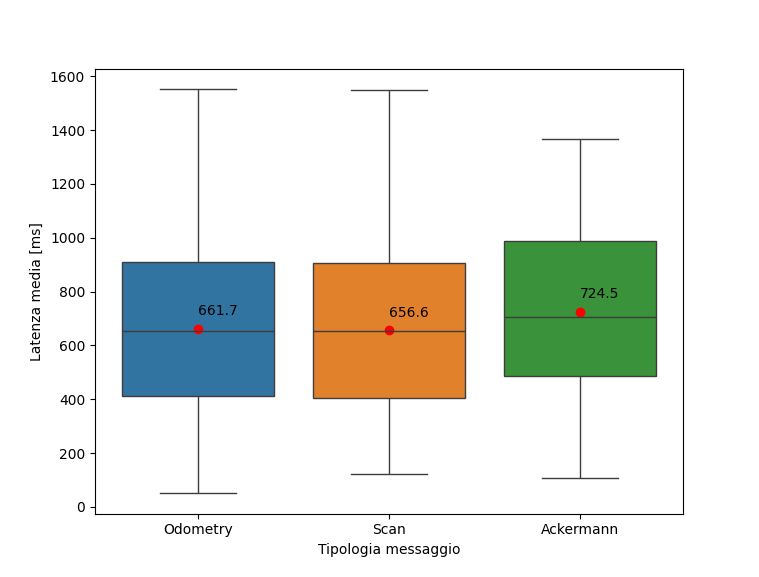
\includegraphics[width=0.7\textwidth]{figures/grafico_latenze.png}
    \caption{Latenze medie dei pacchetti messe a confronto}
    \label{latency_graph}
\end{figure}

\noindent Come è possibile vedere dai dati, mediamente si riscontra una latenza tra i 600 e i 700 millisecondi per quanto riguarda i messaggi dei sensori (odometria e scan), mentre per i messaggi di controllo (ackermann) si riscontrano valori più elevati, tra i 700 e gli 800 millisecondi. Questi alti valori di latenza riscontrati sono dovuti a vari fattori. 

\noindent In primo luogo fra tutti la complessità del protocollo MQTT. Come discusso nella sezione \ref{scelte_progettuali_affidabilità}, le procedure di conferma di ricezione e di ritrasmissione dei messaggi, pur essenziali per garantire la robustezza delle comunicazioni, introducono inevitabilmente ritardi nella trasmissione dei dati.

\noindent In secondo luogo, il mezzo di trasmissione utilizzato, ovvero una rete Wi-Fi, ha limitato le prestazioni del sistema. La tecnologia Wi-Fi, sebbene ampiamente diffusa, presenta caratteristiche intrinseche che possono influenzare negativamente la latenza, come la variabilità del segnale, l'interferenza con altre reti wireless e la saturazione del canale. A differenza di tecnologie più recenti come il 5G, che offrono una banda più elevata e una latenza significativamente inferiore, la rete Wi-Fi può costituire un collo di bottiglia nelle applicazioni che richiedono tempi di risposta estremamente rapidi.

\noindent Il grafico a candela di Figura \ref{latency_graph} evidenzia la notevole variabilità dei tempi di trasmissione. Questa alta instabilità, insieme ai dati in tabella \ref{tabella_latenza} avvalorano l'ipotesi che l'utilizzo di una rete Wi-Fi non sia ottimale per questo tipo di applicazione.

